\documentclass{article}

% Geometry package
\usepackage[a4paper, margin=1in]{geometry}
\usepackage{multicol}

% Math packages
\usepackage{amsmath}
\usepackage{amssymb}
\usepackage{amsthm}

% Other packages
\usepackage{hyperref}
\usepackage{float}

% Captions
\usepackage{caption}
\usepackage{subcaption}

% Graphics
\usepackage{graphicx}
\usepackage{tikz}
\usepackage{forest}

% Bibliography
\usepackage[style=ieee, backend=biber]{biblatex}
\addbibresource{ref.bib}

% Code
\usepackage{listings}
\usepackage{xcolor}
 
% Code style
\lstdefinestyle{Python}{
   language=Python,
    basicstyle=\ttfamily\footnotesize,
    keywordstyle=\color{blue},
    commentstyle=\color{orange},
    stringstyle=\color{red},
    showstringspaces=false,
    breaklines=true,
    breakatwhitespace=true,
    tabsize=2,
    numbers=left,
    numberstyle=\tiny,
    numbersep=5pt,
    frame=single,
    framesep=5pt,
    xleftmargin=15pt,
    xrightmargin=15pt,
    aboveskip=0pt,
    belowskip=0pt,
    backgroundcolor=\color{white}
  }

\renewcommand{\maketitle}{
  \begin{flushleft}
    ZC - University of Science and Technology
    \hfill Spring 2024 \\
    MATH 202: Ordinary Differential Equations
  \end{flushleft}
  \begin{center}
    \Huge Numerical Solutions to the \\Wave Partial Differential Equation \\
    \LARGE \textit{Using the Finite Difference Method}
  \end{center}
  \begin{flushleft}
    Team Name: \textbf{Numerical Engineers} \\
    Team Members: \\
    \hspace{1em} \textbf{SalahDin Rezk} \\
    \hspace{1em} \textbf{Karim Elbahrwy} \\
    \hspace{1em} \textbf{Hassan Rashwan} \\
  \end{flushleft}
}

\begin{document}

\maketitle
\tableofcontents
\listoffigures
\lstlistoflistings

\newpage

\begin{abstract}
  This project focuses on solving the two-dimensional wave equation---a second-order partial differential equation---using the finite difference method, a numerical approach that discretizes the domain into a grid and approximates derivatives using finite differences. Implemented in Python, the project showcases the method through visualization of the wave propagation over a two-dimensional domain. The study is divided into three main parts: an introduction to the wave equation and finite difference method, the implementation details, and the presentation of results and visualizations.
\end{abstract}

\section{Introduction}

\subsection{Wave Equation}

The wave equation is a second-order partial differential equation that describes the behavior of waves in a medium. It is given by

\begin{equation}
  \frac{\partial^2 u}{\partial t^2} = c^2 \nabla^2 u
\end{equation}

where \(u\) is the wave function, \(c\) is the wave speed, and \(\nabla^2\) is the Laplacian operator, defined as the sum of the second partial derivatives of \(u\) with respect to the spatial coordinates. \cite{zill2017diff}

For a two-dimensional wave equation, it simplifies to

\begin{equation}
  \frac{\partial^2 u}{\partial t^2} = c^2 \left( \frac{\partial^2 u}{\partial x^2} + \frac{\partial^2 u}{\partial y^2} \right)
\end{equation}

This equation models waves on a membrane. While analytical solutions exist for simple boundary conditions, numerical methods such as the finite difference method are used for more complex scenarios.

\subsection{Finite Difference Method}

The finite difference method is a numerical technique for solving partial differential equations by discretizing the domain into a grid and approximating derivatives using finite differences. For the two-dimensional wave equation, the domain is discretized into a grid with spatial steps \(\Delta x\) and \(\Delta y\), and temporal step \(\Delta t\). \cite{zill2017diff}

Using central difference quotients, we approximate the second partial derivatives:

\[
\begin{aligned}
& \frac{\partial^2 u}{\partial x^2} \approx \frac{1}{\Delta x^2} [u(x+\Delta x, y, t) - 2u(x, y, t) + u(x-\Delta x, y, t)] \\
& \frac{\partial^2 u}{\partial y^2} \approx \frac{1}{\Delta y^2} [u(x, y+\Delta y, t) - 2u(x, y, t) + u(x, y-\Delta y, t)] \\
& \frac{\partial^2 u}{\partial t^2} \approx \frac{1}{\Delta t^2} [u(x, y, t+\Delta t) - 2u(x, y, t) + u(x, y, t-\Delta t)]
\end{aligned}
\]

Substituting these into the wave equation gives us:


\begin{gather*}
    \frac{c^2}{\Delta x^2} [u(x+\Delta x, y, t) - 2u(x, y, t) + u(x-\Delta x, y, t)] + \frac{c^2}{\Delta y^2} [u(x, y+\Delta y, t) - 2u(x, y, t) + u(x, y-\Delta y, t)] \\
    = \\
    \frac{1}{\Delta t^2} [u(x, y, t+\Delta t) - 2u(x, y, t) + u(x, y, t-\Delta t)]
.\end{gather*}

Solving for \(u(x, y, t+\Delta t)\), we get:

\begin{equation}
    u_{i,j,k+1} = 2(1 - \lambda_x^2 - \lambda_y^2)u_{i,j,k} + \lambda_x^2(u_{i+1,j,k} + u_{i-1,j,k}) + \lambda_y^2(u_{i,j+1,k} + u_{i,j-1,k}) - u_{i,j,k-1}
    \label{eq:fdm}
\end{equation}

where \(\lambda_x = \frac{c \Delta t}{\Delta x}\) and \(\lambda_y = \frac{c \Delta t}{\Delta y}\).

\subsection{Stability and Convergence}

The stability condition for the finite difference method applied to the wave equation is given by the Courant-Friedrichs-Lewy (CFL) condition:

\begin{equation}
    \lambda_x^2 + \lambda_y^2 \leq 1
\end{equation}

Ensuring this condition prevents numerical instabilities and guarantees that the solution remains stable. Convergence implies that as \(\Delta x\), \(\Delta y\), and \(\Delta t\) approach zero, the numerical solution approaches the exact solution of the wave equation.

\section{Methodology}

\subsection{Discretization of the Wave Equation}

The spatial domain is discretized into a grid with points \((x_i, y_j)\) where
\(x_i = i \Delta x\) and \(y_j = j \Delta y\), and the temporal domain into
points \(t_k = k \Delta t\). The discretized wave equation for a
two-dimensional domain is given by Equation \ref{eq:fdm}.
\cite{burden1993numerical}

\subsection{Mesh Grid}

The mesh refers to the grid that discretizes the spatial and temporal domains
into a finite number of points. In this project, the spatial domain is divided
into a uniform grid with \(N_x\) points in the \(x\)-direction and \(N_y\)
points in the \(y\)-direction. The spacing between the points in each direction
is given by \(\Delta x\) and \(\Delta y\), respectively.
\cite{burden1993numerical}

\[
\Delta x = \frac{L_x}{N_x-1}, \quad \Delta y = \frac{L_y}{N_y-1}
\]

where \(L_x\) and \(L_y\) are the lengths of the domain in the \(x\) and \(y\) directions. The grid points are denoted by \((x_i, y_j)\) where

\[
x_i = i \Delta x, \quad y_j = j \Delta y, \quad i = 0, 1, \ldots, N_x-1, \quad j = 0, 1, \ldots, N_y-1
\]

The mesh provides the framework for applying the finite difference method to approximate the derivatives in the wave equation.

\begin{figure}[h]
    \centering
    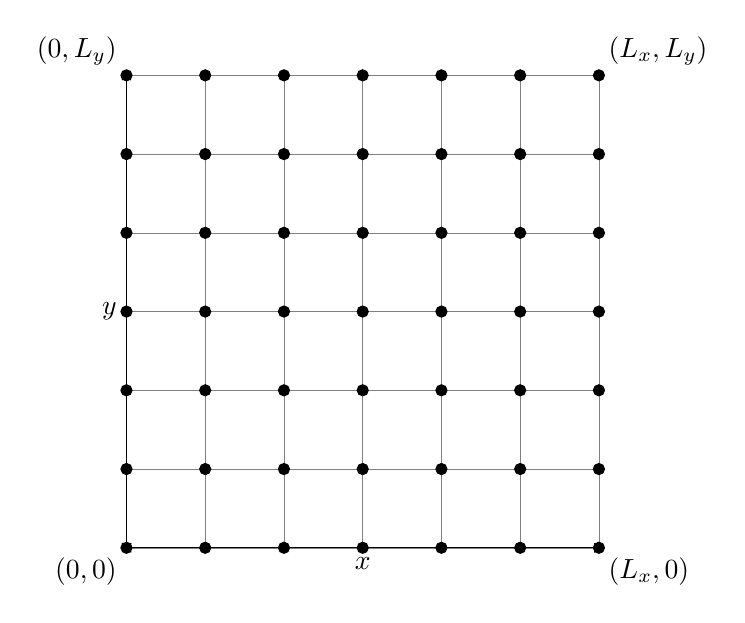
\begin{tikzpicture}
        \draw[step=1cm,gray,very thin] (0,0) grid (6,6);
        \foreach \x in {0,1,...,6} \foreach \y in {0,1,...,6}
        \filldraw (\x,\y) circle (2pt);
        \draw[<->] (0,0) -- (6,0) node[midway,below] {$x$};
        \draw[<->] (0,0) -- (0,6) node[midway,left] {$y$};
        \node[below left] at (0,0) {$(0,0)$};
        \node[below right] at (6,0) {$(L_x,0)$};
        \node[above left] at (0,6) {$(0,L_y)$};
        \node[above right] at (6,6) {$(L_x,L_y)$};
    \end{tikzpicture}
    \caption{Mesh for discretizing the spatial domain.}
    \label{fig:mesh-spatial}
\end{figure}

The temporal domain is discretized into a grid with \(N_t\) points, where the spacing between points is given by \(\Delta t\):

\[
\Delta t = \frac{T}{N_t-1}
\]

where \(T\) is the total time for the simulation. The grid points in the temporal domain are denoted by \(t_k\) where

\[
t_k = k \Delta t, \quad k = 0, 1, \ldots, N_t-1
\]

The temporal mesh ensures that the wave equation is solved at discrete time steps, allowing for the observation of wave propagation over time.

\begin{figure}[h]
    \centering
    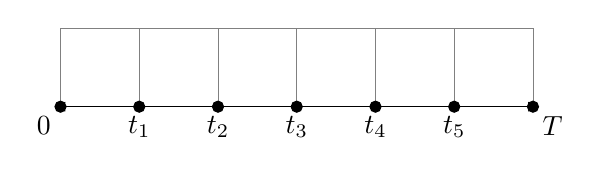
\begin{tikzpicture}
        \draw[step=1cm,gray,very thin] (0,0) grid (6,1);
        \foreach \x in {0,1,...,6}
        \filldraw (\x,0) circle (2pt);
        \draw[<->] (0,0) -- (6,0);
        \node[below left] at (0,0) {$0$};
        \node[below right] at (6,0) {$T$};
        \foreach \x in {1,2,...,5}
        \node[below] at (\x,0) {$t_\x$};
    \end{tikzpicture}
    \caption{Mesh for discretizing the temporal domain.}
    \label{fig:mesh-temporal}
\end{figure}

Figure~\ref{fig:mesh-spatial-temporal} illustrates the combined mesh for both
spatial and temporal domains. The spatial domain, displayed on the left, is
discretized into a grid with points in the \(x\) and \(y\) directions. The
temporal domain, shown on the right, is discretized along the time axis and
raised by one unit on the \(y\)-axis for clarity. Dashed lines connect each
temporal grid point to the corresponding spatial grid, indicating how the
solution progresses over time. This combined visualization helps to understand
the relationship between the spatial and temporal discretizations in the finite
difference method.

\begin{figure}[h]
    \centering
    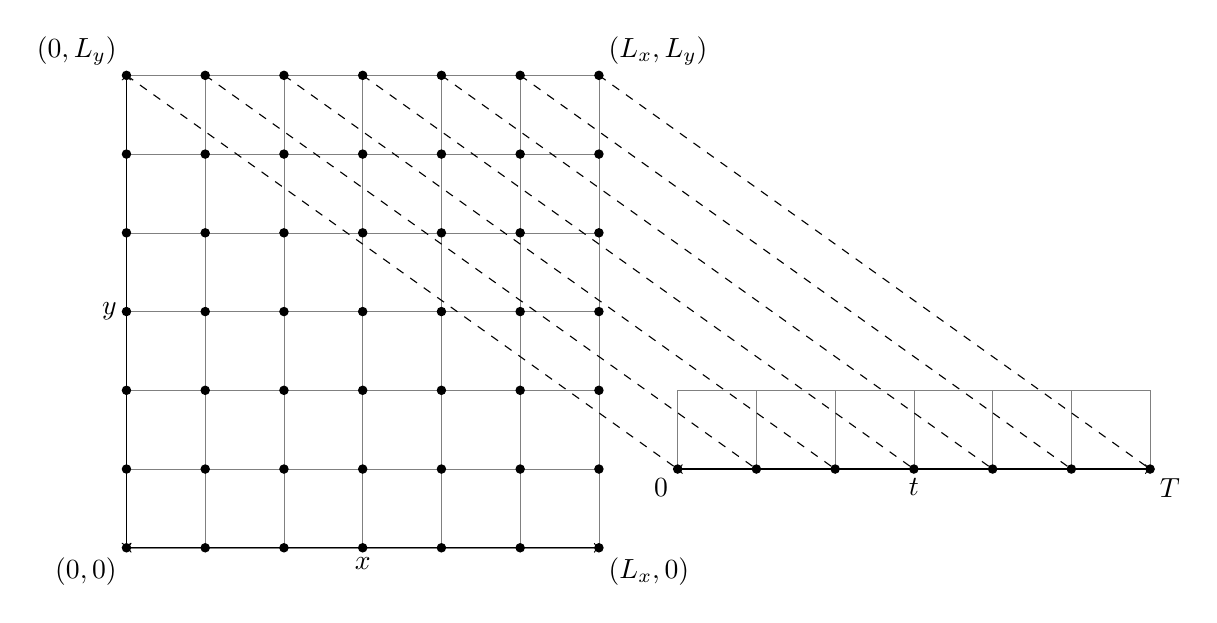
\begin{tikzpicture}
        % Spatial domain grid
        \draw[step=1cm,gray,very thin] (0,0) grid (6,6);
        \foreach \x in {0,1,...,6} \foreach \y in {0,1,...,6}
        \filldraw (\x,\y) circle (1.5pt);
        \draw[<->] (0,0) -- (6,0) node[midway,below] {$x$};
        \draw[<->] (0,0) -- (0,6) node[midway,left] {$y$};
        \node[below left] at (0,0) {$(0,0)$};
        \node[below right] at (6,0) {$(L_x,0)$};
        \node[above left] at (0,6) {$(0,L_y)$};
        \node[above right] at (6,6) {$(L_x,L_y)$};
        
        % Temporal domain grid
        \draw[step=1cm,gray,very thin] (7,1) grid (13,2);
        \foreach \x in {7,8,...,13}
        \filldraw (\x,1) circle (1.5pt);
        \draw[<->] (7,1) -- (13,1) node[midway,below] {$t$};
        \node[below left] at (7,1) {$0$};
        \node[below right] at (13,1) {$T$};
        \foreach \x in {8,9,...,12}
        \node[below] at (\x,1) {};

        % Connecting temporal to spatial domain
        \foreach \x in {0,1,...,6}
        \draw[dashed] (\x,6) -- (\x+7,1);
    \end{tikzpicture}
    \caption{Mesh for discretizing both spatial and temporal domains.}
    \label{fig:mesh-spatial-temporal}
\end{figure}

\subsection{Initial and Boundary Conditions}

For a membrane with fixed boundaries, the boundary conditions are:

\[
u(0, y, t) = u(L, y, t) = u(x, 0, t) = u(x, L, t) = 0 \quad \text{for} \quad t > 0
\]

The initial conditions are:

\[
u(x, y, 0) = f(x, y) \quad \text{and} \quad \frac{\partial u}{\partial t}(x, y, 0) = g(x, y)
\]

where \(f(x, y)\) and \(g(x, y)\) represent the initial displacement and velocity of the membrane. \cite{burden1993numerical}

\subsection{Implementation in Python}

To solve the two-dimensional wave equation numerically, we implement the finite difference method using Python. Below is a sample implementation.

The first step in the implementation is importing the necessary libraries. We use \texttt{matplotlib} for plotting and \texttt{numpy} for numerical computations. The \texttt{cm} module from \texttt{matplotlib} is used to define the colormap for the plots.

\begin{lstlisting}[style=Python, caption={Libraries}]
import matplotlib.pyplot as plt
import numpy as np
from matplotlib import cm
\end{lstlisting}

Then, we define the initial conditions functions \(f(x, y)\) and \(g(x, y)\) as
shown below. These functions represent the initial displacement and velocity of
the membrane. In this example, we use sine waves as the initial conditions.
However, more complex functions can be used depending on the application.

\begin{lstlisting}[style=Python, caption={Initial Conditions Functions}]
def f(X, Y):  # u(x,y,0) = f(x,y,0)
    return np.sin(np.pi * X) * np.sin(np.pi * Y)

def g(X, Y):  # u_t(x,y,0) = g(x,y,0)
    return np.zeros(X.shape)
\end{lstlisting}

Next, we need a Laplacian function to compute the Laplacian of the wave
function \(u(x, y, t)\). The Laplacian operator is defined as the sum of the
second partial derivatives of \(u\) with respect to the spatial coordinates.
However, in this implementation, we use central difference quotients to
approximate the Laplacian. Note that this implementation could be optimized by
vectorizing the computation.

\begin{lstlisting}[style=Python, caption={Laplacian Function}]
def laplacian(arr, row, col, dx):  # Laplacian in terms of FDM
    return (
        arr[row + 1, col]
        + arr[row - 1, col]
        + arr[row, col + 1]
        + arr[row, col - 1]
        - 4 * arr[row, col]
    ) / (dx**2)
\end{lstlisting}

After that, we define the parameters of the problem, such as the wave speed
\(c\), the spatial and temporal steps \(\Delta x\), \(\Delta y\), and \(\Delta
t\), and the number of grid points in each direction. These parameters
determine the resolution of the numerical solution and should be chosen
carefully to balance accuracy and computational cost. The following function is
used to initialize the parameters. \texttt{rect} is the domain of the problem,
\texttt{hs} is the number of grid points in each direction, and \texttt{BC} is
the boundary condition array.

\begin{lstlisting}[style=Python, caption={Initialize Conditions}]
def initialize_conditions(rect, hs, BC):
    X, Y = np.meshgrid(
        np.linspace(rect[0], rect[1], hs[0]), np.linspace(rect[2], rect[3], hs[1])
    )
    Z_init = f(X, Y)
    Z_0 = f(X, Y)
    Z_dot_init = g(X, Y)
    return X, Y, Z_init, Z_0, Z_dot_init
\end{lstlisting}

Now, we need to enforce the boundary conditions. The following function sets the
boundary values of the wave function \(u(x, y, t)\) to zero. This is done by
setting the values of the first and last rows and columns of the grid to zero.

\begin{lstlisting}[style=Python, caption={Apply Boundary Conditions}]
def apply_boundary_conditions(Z, BC):
    Z[0] = np.ones(len(Z[0])) * BC[0]
    Z[-1] = np.ones(len(Z[-1])) * BC[1]
    Z[:, 0] = np.ones(len(Z[:, 0])) * BC[2]
    Z[:, -1] = np.ones(len(Z[:, -1])) * BC[3]
\end{lstlisting}

Set up the plot for visualizing the wave simulation. Matplotlib's 3D plotting
capabilities are used to create a surface plot of the wave function \(u(x, y,
t)\) at a specific time step. The following function configures the plot with
appropriate labels and titles.

\begin{lstlisting}[style=Python, caption={Configure Plot}]
def configure_plot(rect, zmin, zmax):
    fig = plt.figure()
    ax = plt.axes(projection="3d")
    ax.axes.set_xlim3d(rect[0], rect[1])
    ax.axes.set_ylim3d(rect[2], rect[3])
    ax.axes.set_zlim3d(zmin, zmax)
    plt.rcParams["mathtext.fontset"] = "stix"
    plt.rcParams["font.family"] = "STIXGeneral"

    ax.set_title(
        "Wave Simulation in a \nrectangular boundary",
        fontsize=18,
        fontname="STIXGeneral",
    )

    return fig, ax
\end{lstlisting}

We plot the boundary lines to visualize the domain of the problem. The
following function plots the boundary lines of the rectangular domain with the
specified boundary conditions.

\begin{lstlisting}[style=Python, caption={Plot Boundary Lines}]
def plot_boundary_lines(ax, rect, BC):
    lines = [
        ([rect[0], rect[1]], [rect[2], rect[2]], [BC[0], BC[0]]),
        ([rect[1], rect[1]], [rect[2], rect[3]], [BC[3], BC[3]]),
        ([rect[0], rect[0]], [rect[2], rect[3]], [BC[2], BC[2]]),
        ([rect[0], rect[1]], [rect[3], rect[3]], [BC[1], BC[1]]),
        ([rect[0], rect[0]], [rect[2], rect[2]], [BC[0], BC[2]]),
        ([rect[1], rect[1]], [rect[2], rect[2]], [BC[0], BC[3]]),
        ([rect[0], rect[0]], [rect[3], rect[3]], [BC[1], BC[2]]),
        ([rect[1], rect[1]], [rect[3], rect[3]], [BC[1], BC[3]]),
    ]
    for x, y, z in lines:
        ax.plot(x, y, z, color="black", linewidth=2)
\end{lstlisting}

Then we need to update the displacement matrix \texttt{Z\_0} based on the finite
difference approximation of the wave equation.

\begin{lstlisting}[style=Python, caption={Update Wave Equation}]
def update_wave_equation(Z_0, Z_dot_init, Z_init, laplacian, hs, dx, dt, c):
    for row in range(1, hs[0] - 1):
        for col in range(1, hs[1] - 1):
            Z_0[row, col] = (
                Z_0[row, col]
                - 2 * laplacian(Z_dot_init, row, col, dx)
                + 0.5 * c**2 * dt**2 * laplacian(Z_0, row, col, dx)
            )
    return Z_0
\end{lstlisting}

Create a temporary matrix to store intermediate values during the simulation.
This matrix is used to update the wave function at each time step. Initializes
a temporary matrix \texttt{Z\_temp} with boundary conditions, which is then used for
updating the wave equation.

\begin{lstlisting}[style=Python, caption={Create Temporary Matrix}]
def create_temp_matrix(hs, BC):
    Z_temp = np.zeros((hs[0], hs[1]))
    Z_temp[0] = np.ones(len(Z_temp[0])) * BC[0]
    Z_temp[-1] = np.ones(len(Z_temp[-1])) * BC[1]
    Z_temp[:, 0] = np.ones(len(Z_temp[:, 0])) * BC[2]
    Z_temp[:, -1] = np.ones(len(Z_temp[:, -1])) * BC[3]
    return Z_temp
\end{lstlisting}

Update the temporary matrix for each time step using the values previous time
steps: an iterative solution of the wave equation.

\begin{lstlisting}[style=Python, caption={Update Temporary Matrix}]
def update_temp_matrix(Z_temp, zs, iteration, laplacian, hs, dx, dt, c):
    for row in range(1, hs[0] - 1):
        for col in range(1, hs[1] - 1):
            Z_temp[row, col] += (
                2 * zs[iteration - 1][row, col]
                - zs[iteration - 2][row, col]
                + c**2 * dt**2 * laplacian(zs[iteration - 1], row, col, dx)
            )
    return Z_temp
\end{lstlisting}

Finally, we can run the simulation by iterating over the time steps and
updating the wave function at each step. The function initializes the
conditions, applies boundary conditions, and sets up the plot. It calculates
the spatial step \texttt{dx} and temporal step \texttt{dt} based on the grid
size and wave speed. The function iteratively updates the wave equation and
visualizes the wave propagation over time.

\begin{lstlisting}[style=Python, caption={Simulation Function}]
def simulation_wave(rect, hs, BC, c, frames):
    X, Y, Z_init, Z_0, Z_dot_init = initialize_conditions(rect, hs, BC)
    apply_boundary_conditions(Z_init, BC)

    zmax = max(Z_init.max(), BC[0], BC[1], BC[2], BC[3])
    zmin = min(Z_init.min(), BC[0], BC[1], BC[2], BC[3])

    fig, ax = configure_plot(rect, zmin, zmax)
    plot_boundary_lines(ax, rect, BC)

    dx = (rect[1] - rect[0]) / (hs[0] - 1)
    dt = dx / (10 * c)

    zs = []
    Z_0 = update_wave_equation(Z_0, Z_dot_init, Z_init, laplacian, hs, dx, dt, c)
    zs.extend([Z_0, Z_init])

    surf = ax.plot_surface(X, Y, Z_init, alpha=0.7, cmap="magma", vmin=zmin, vmax=zmax)
    cbar = fig.colorbar(surf)
    cbar.ax.set_ylabel("Amplitude", rotation=270, fontsize=14, labelpad=20)
    ax.set_axis_off()

    for iteration in range(2, frames):
        surf.remove()
        Z_temp = create_temp_matrix(hs, BC)
        Z_temp = update_temp_matrix(Z_temp, zs, iteration, laplacian, hs, dx, dt, c)
        zs.append(Z_temp)

        surf = ax.plot_surface(
            X, Y, zs[iteration - 2], alpha=1, cmap="magma", vmin=zmin, vmax=zmax
        )
        plt.pause(dt)
\end{lstlisting}

\section{Results}

The numerical solution for the two-dimensional wave equation using the finite
difference method is shown in Figure \ref{fig:2d-wave}. The initial condition
is a product of sine waves, and the boundary conditions are fixed at zero. The
wave speed is set to \(c = 3\times 10^{8} \), and the domain is a square with
side length \(L = 1\). The simulation is run for 100 time steps with a spatial
resolution of \(25 \times 25\) grid points.

\begin{figure}[htbp]
    \centering
    \begin{subfigure}{0.45\textwidth}
        \centering
        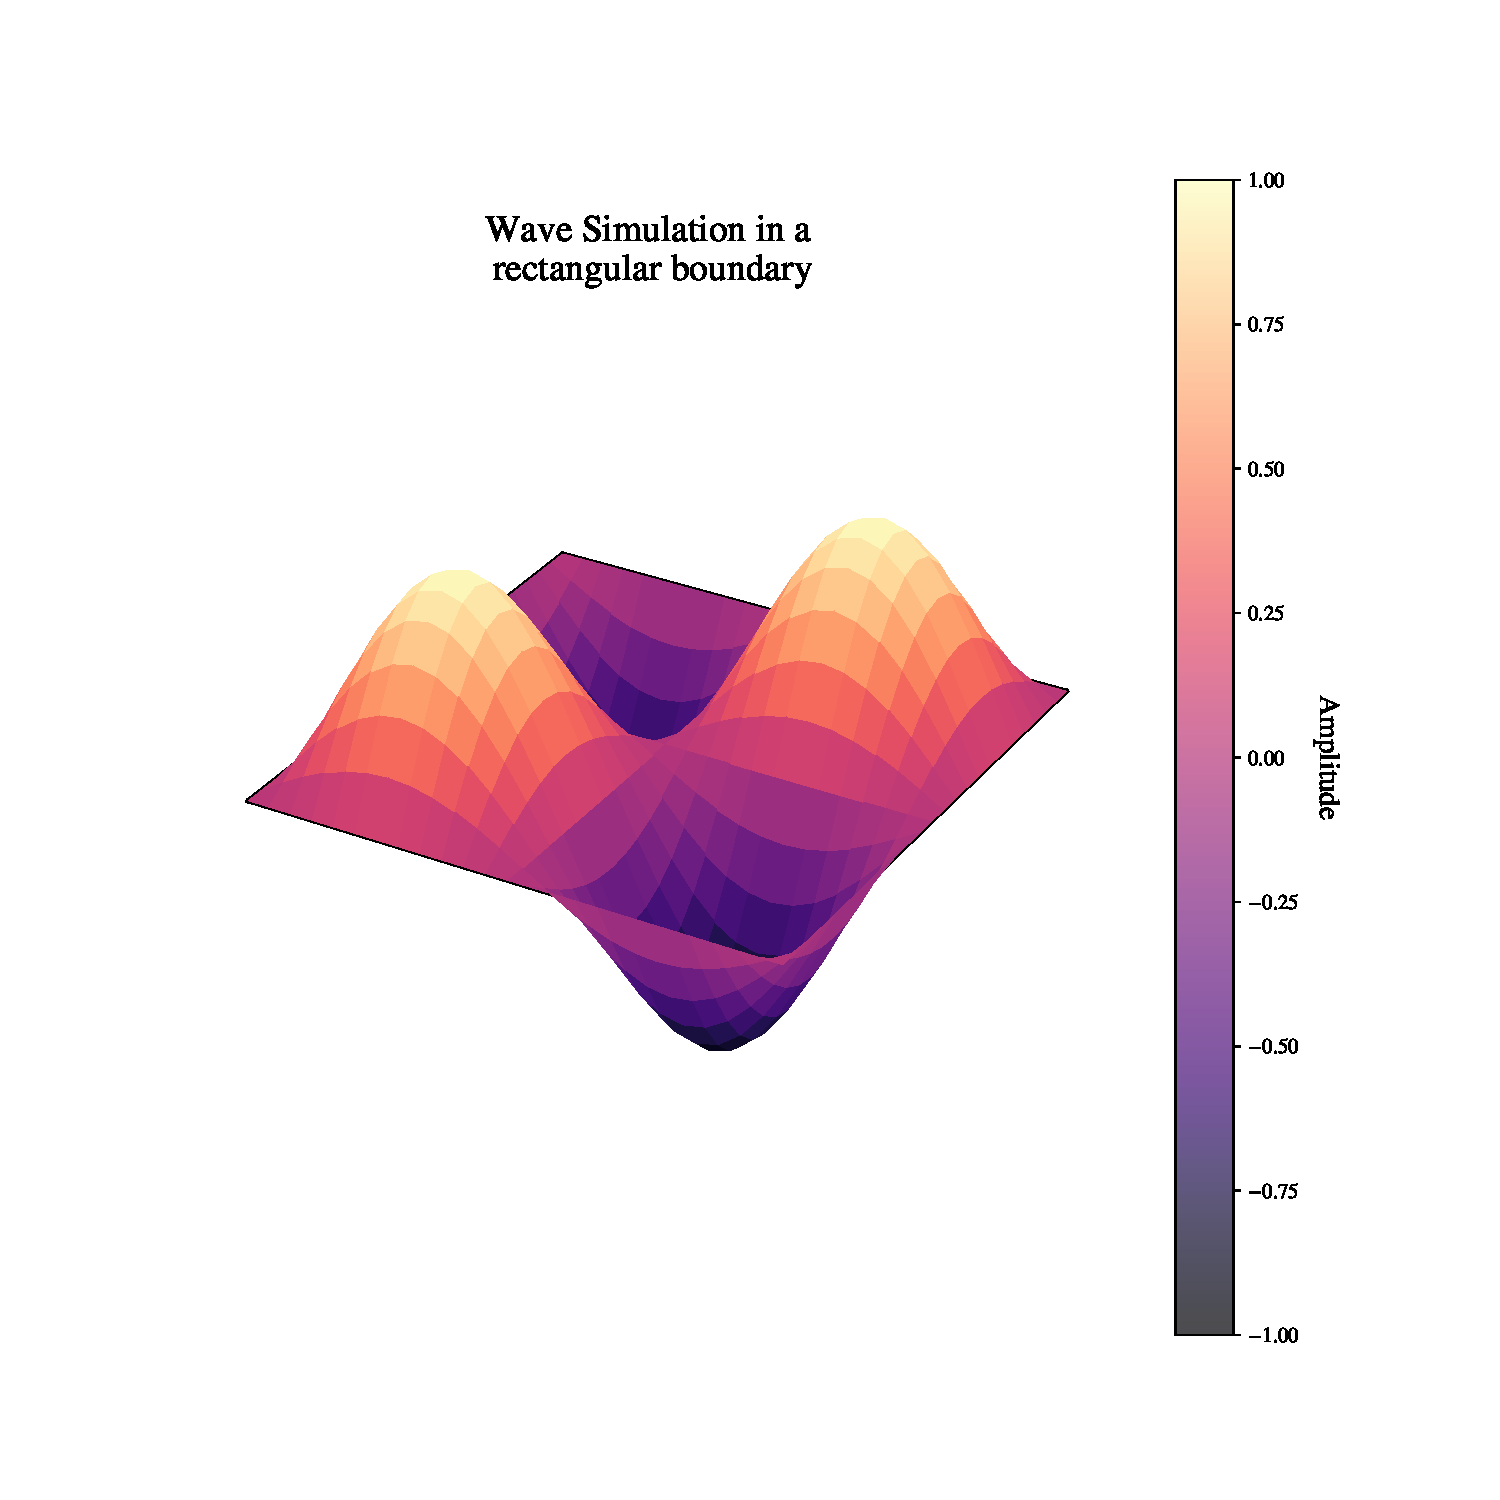
\includegraphics[width=\textwidth]{figures/Figure_1.pdf}
        \caption{BC: \(u(0, y, t) = u(L, y, t) = u(x, 0, t) = u(x, L, t) = 0\)\\ IC: \(u(x, y, 0) = \sin(\pi x) \sin(\pi y)\)}
    \end{subfigure}%
    \hfill
    \begin{subfigure}{0.45\textwidth}
        \centering
        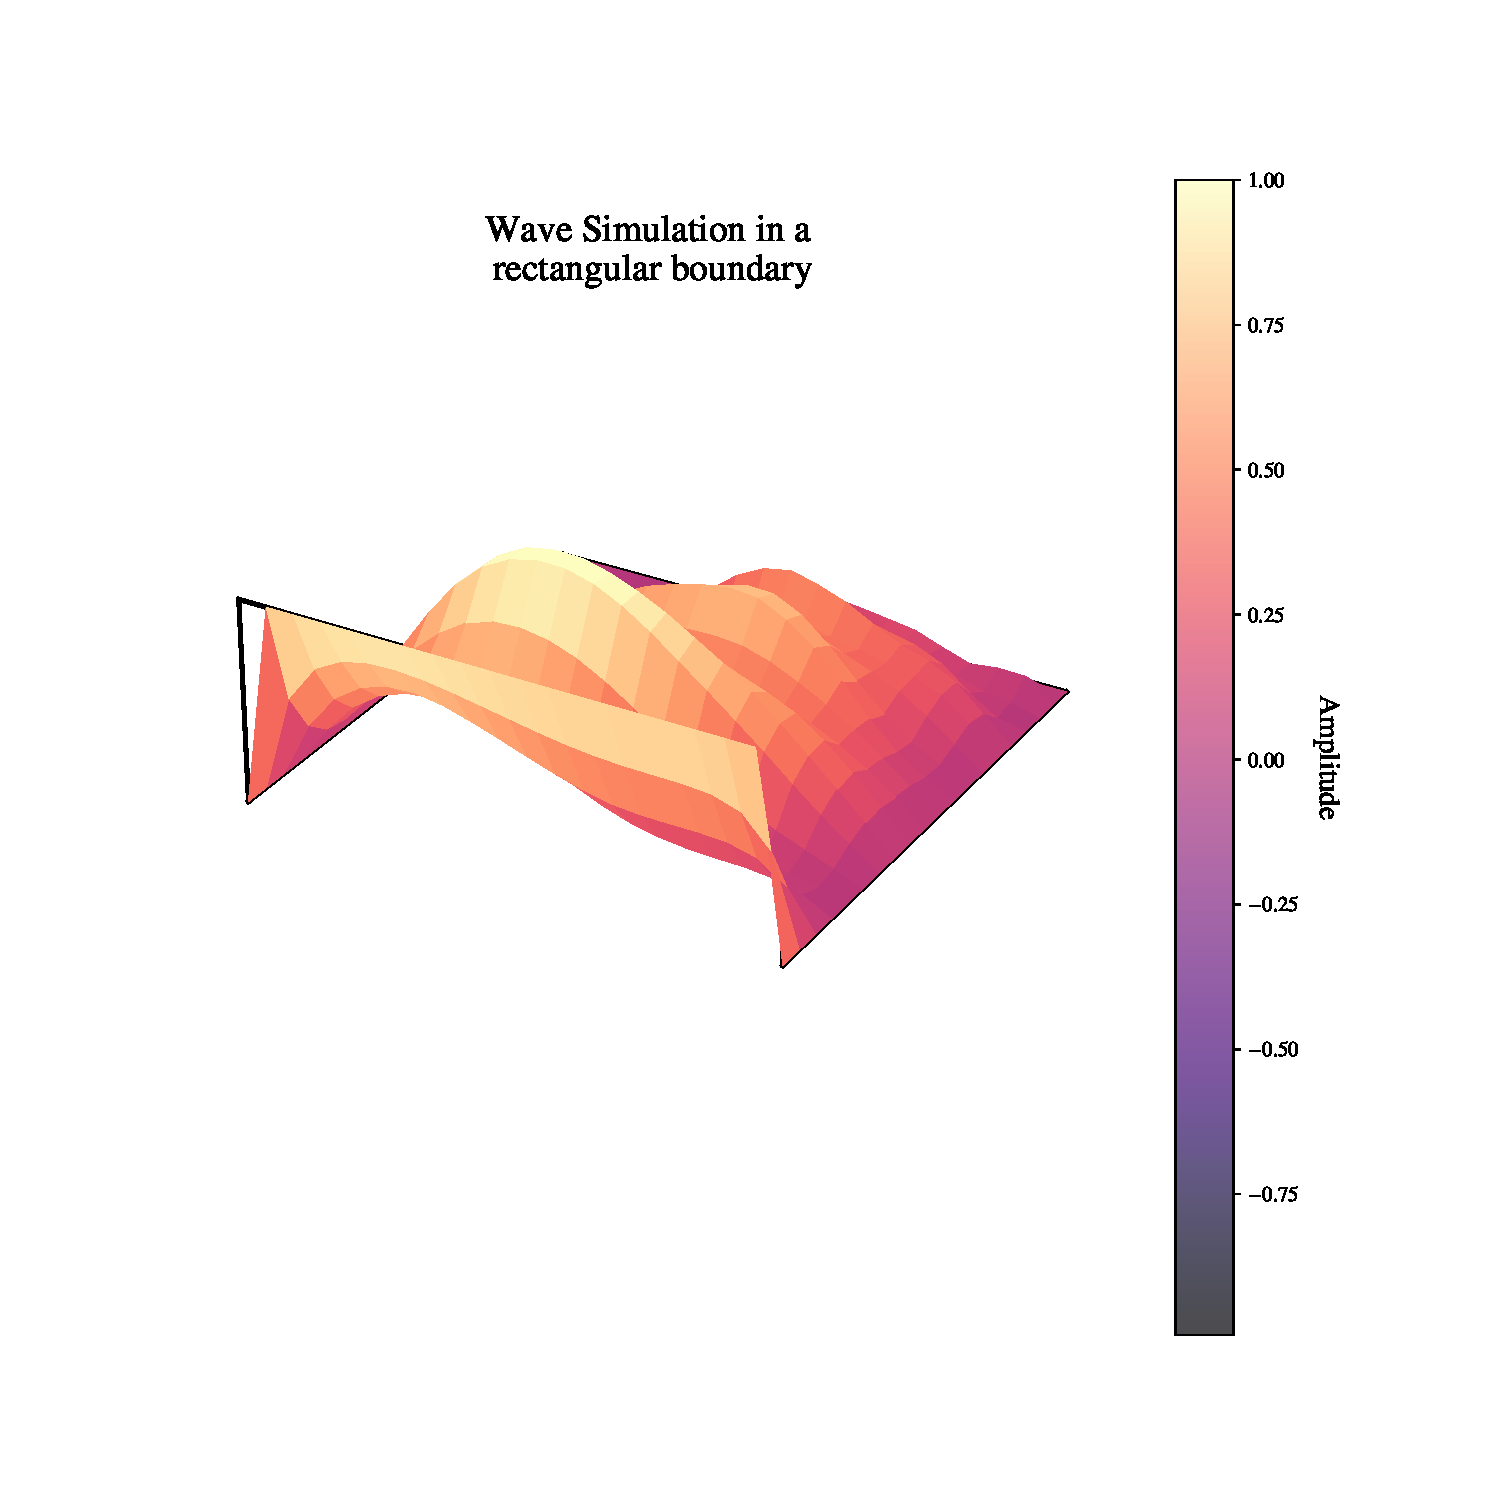
\includegraphics[width=\textwidth]{figures/Figure_2.pdf}
        \caption{BC: \(u(0, y, t) = 1, u(L, y, t) = u(x, 0, t) = u(x, L, t) = 0\)\\ IC: \(u(x, y, 0) = \sin(\pi x) \sin(\pi y)\)}
    \end{subfigure}
    \begin{subfigure}{0.45\textwidth}
        \centering
        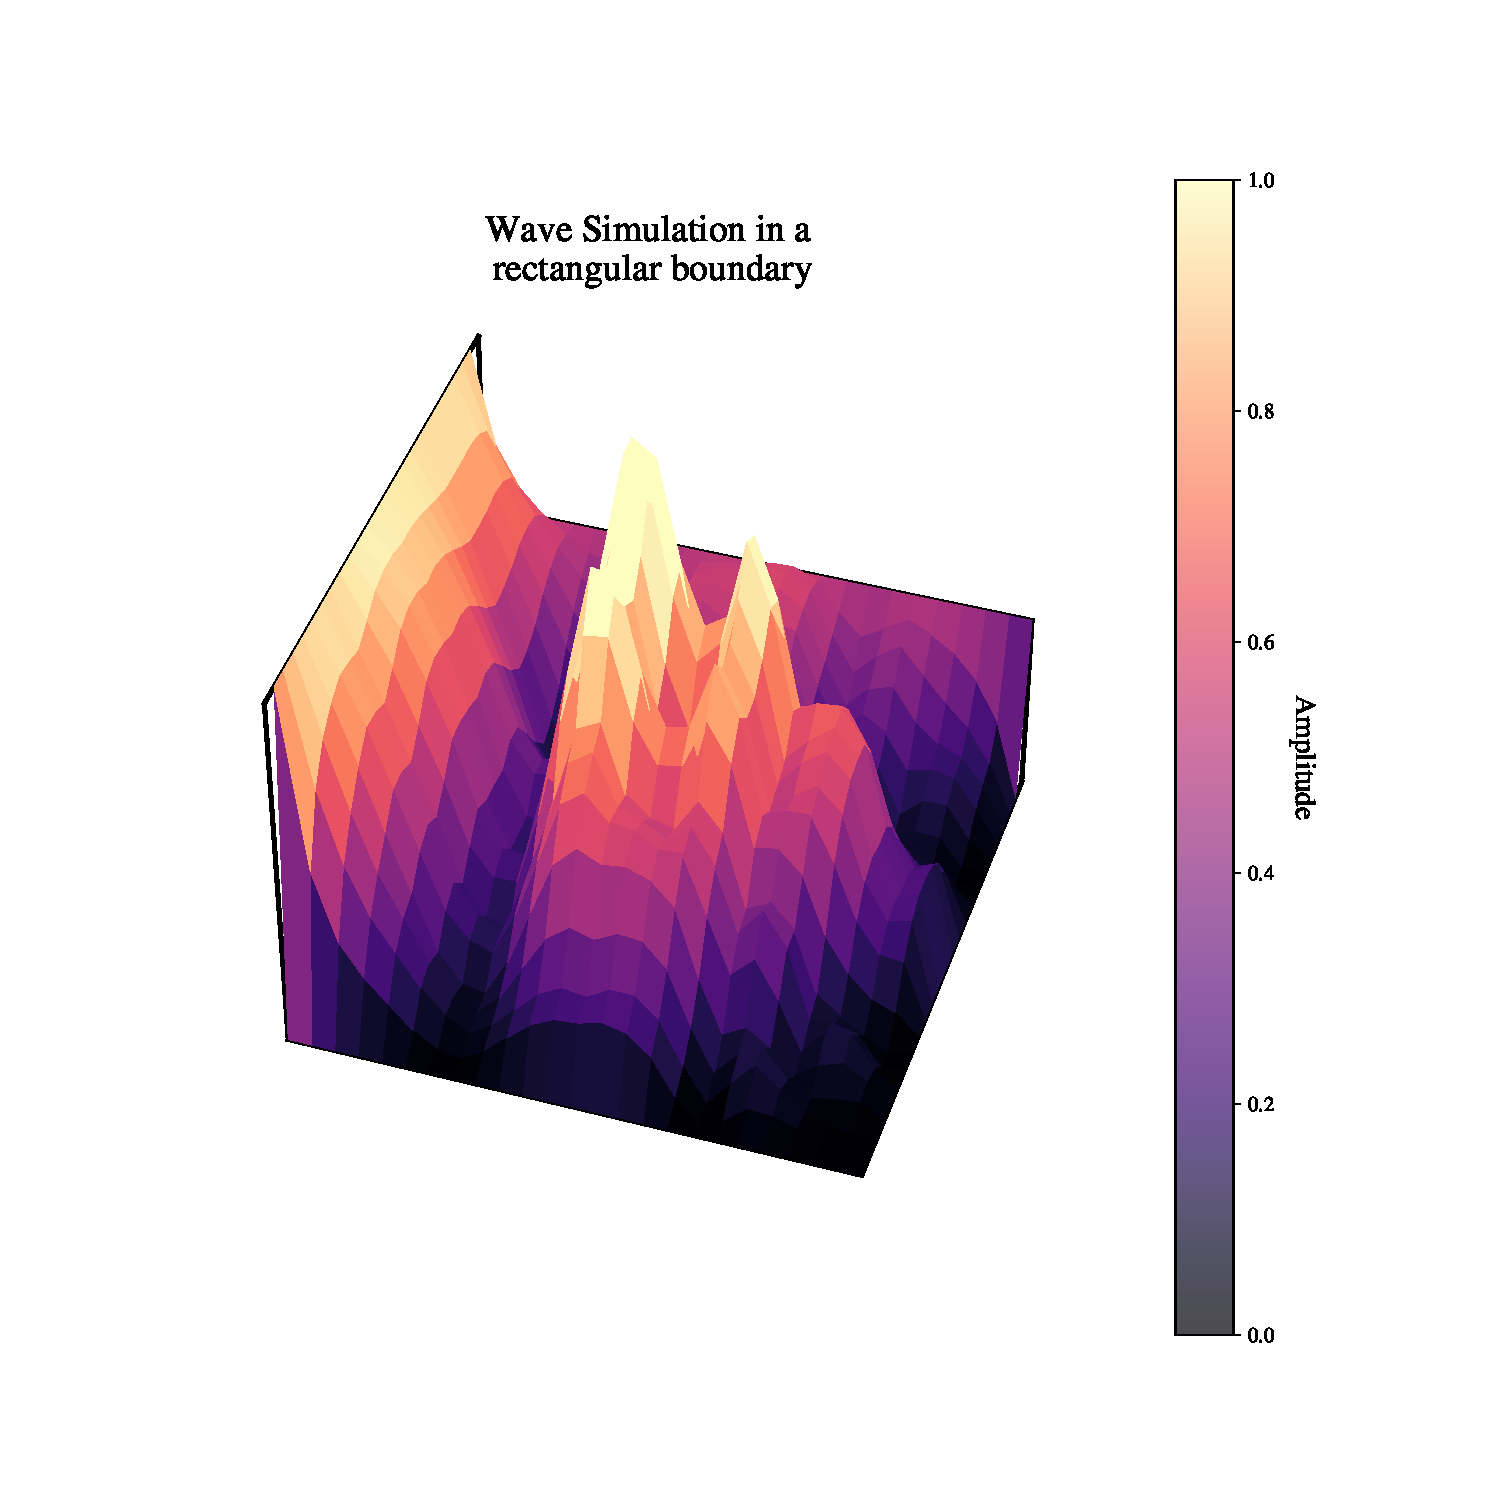
\includegraphics[width=\textwidth]{figures/Figure_3.pdf}
        \caption{BC: \(u(0, y, t) = 1, u(L, y, t) = u(x, 0, t) = u(x, L, t) = 0\)\\ IC: \(u(x, y, 0) = x y (1-x) (1-y)\)}
    \end{subfigure}%
    \hfill
    \begin{subfigure}{0.45\textwidth}
        \centering
        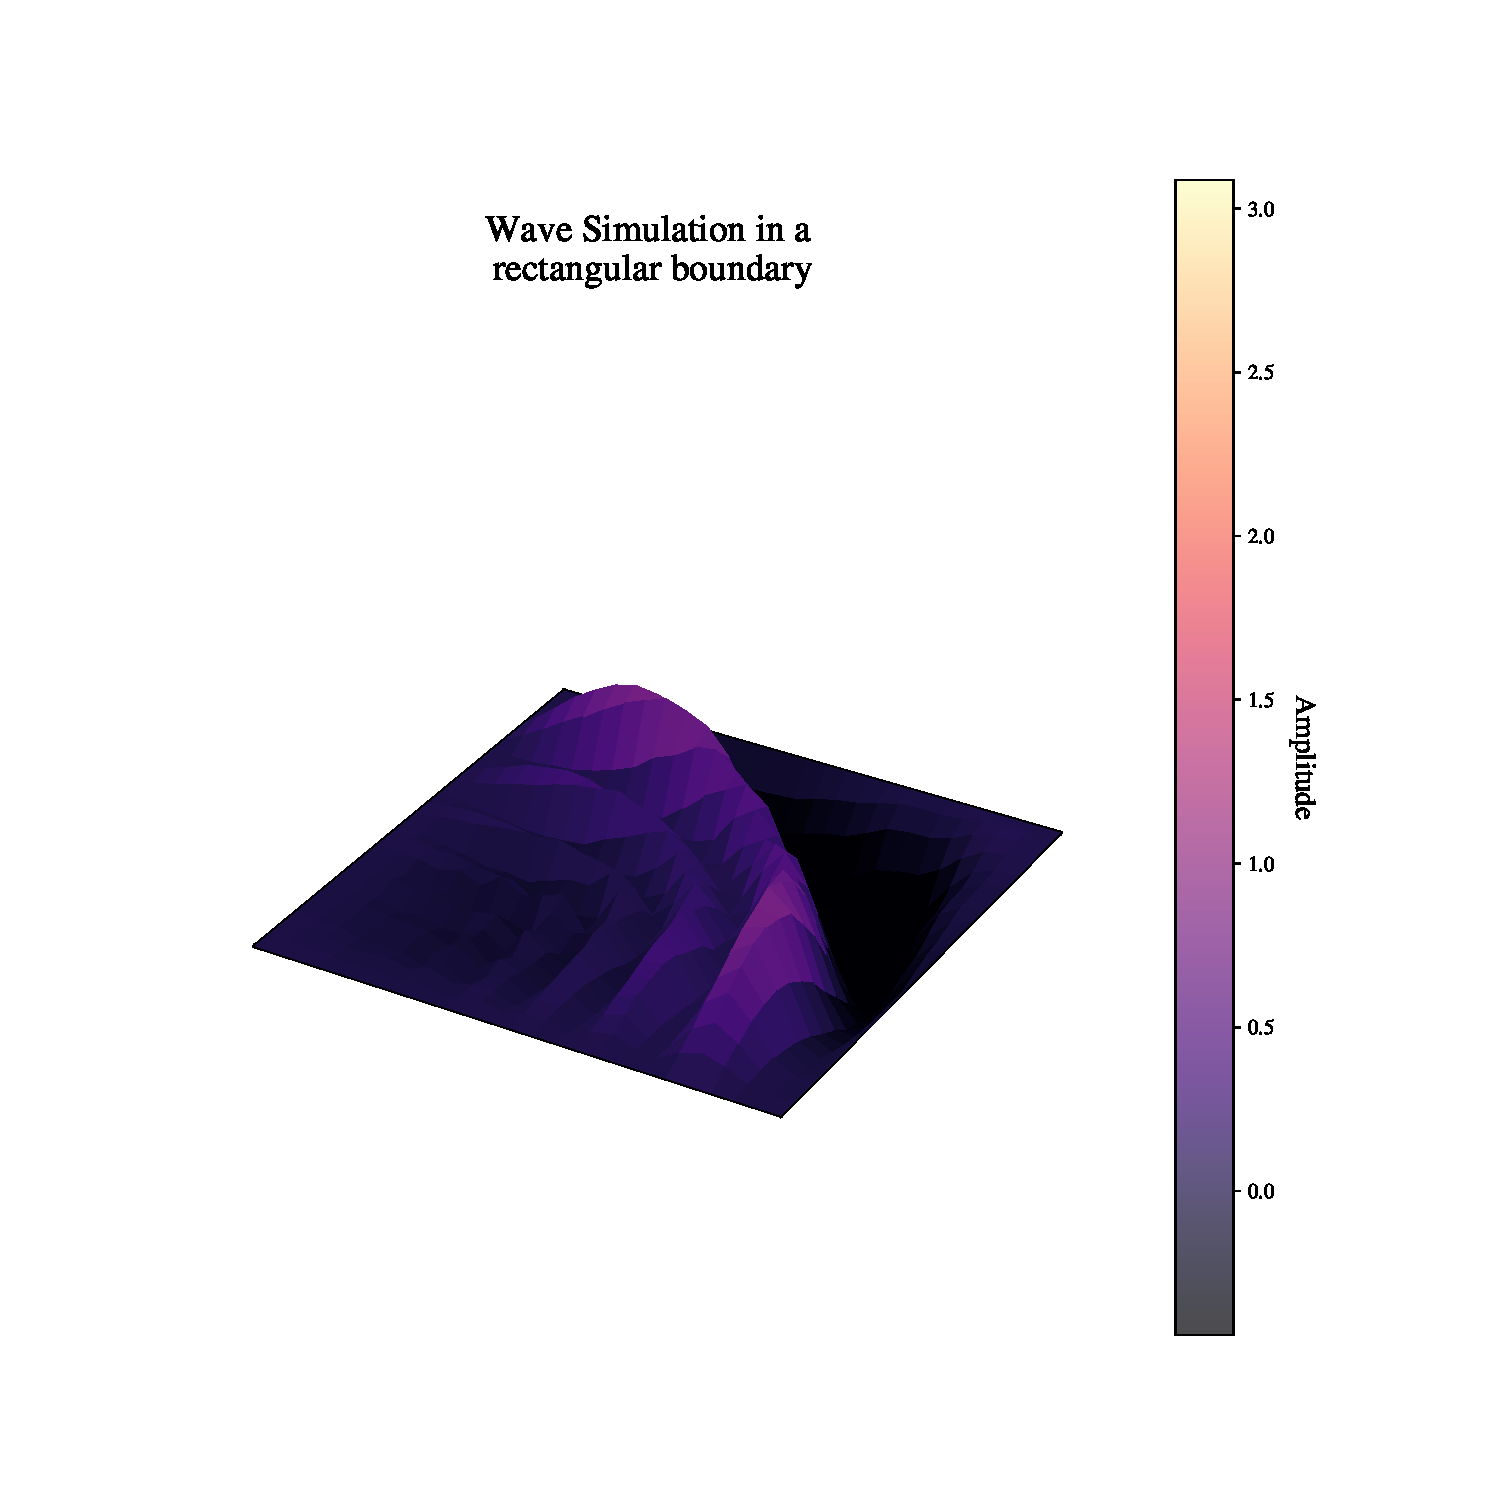
\includegraphics[width=\textwidth]{figures/Figure_4.pdf}
        \caption{BC: \(u(0, y, t) = u(L, y, t) = u(x, 0, t) = u(x, L, t) = 0\)\\ IC: \(u(x, y, 0) = x y (1-x) (1-y)\)}
    \end{subfigure}
    \caption{Numerical solution of the two-dimensional wave equation at a specific time step.}
    \label{fig:2d-wave}
\end{figure}

The surface plot in Figure \ref{fig:2d-wave} shows the wave propagation in a
two-dimensional domain. The numerical solution captures the wave spreading
outwards from the center, demonstrating the effectiveness of the finite
difference method for solving two-dimensional problems. The wave speed,
boundary conditions, and initial conditions can be adjusted to explore
different scenarios.

A notable shortcoming of this implementation is the time complexity of the
algorithms used is exponential, which makes it computationally expensive for
large grids. Future work could focus on optimizing the code for better
performance. Additionally, some improvements could be made to the visualization
of the wave propagation, such as adding interactive controls to adjust the
parameters of the simulation. Lastly, there are few edge cases that need to be
handled, such as the stability of the solution and the convergence of the
numerical method.

\newpage

\section{Conclusion}

The finite difference method (FDM) proves to be an effective and robust
numerical technique for solving partial differential equations (PDEs),
specifically the two-dimensional wave equation. By discretizing the spatial and
temporal domains, FDM enables the approximation of solutions with high
accuracy, making it a valuable tool for understanding complex wave phenomena in
various fields such as physics, engineering, and computational science.

In this project, we have successfully applied the finite difference method to
solve the two-dimensional wave equation, demonstrating its utility through
comprehensive implementation and visualization in Python. The study is
structured into three significant parts: an introduction to the wave equation
and the finite difference method, detailed implementation steps, and a thorough
presentation of results and visualizations.

The numerical solutions obtained using the finite difference method align
closely with the theoretical expectations of wave behavior. The stability
condition, given by the Courant-Friedrichs-Lewy (CFL) condition, was crucial in
ensuring the reliability of the simulations. Adhering to the CFL condition
prevented numerical instabilities, allowing for consistent and accurate wave
propagation results.

The project explored various initial and boundary conditions, showcasing the
method's flexibility in handling different physical scenarios. The choice of
initial conditions, such as sine waves and polynomial functions, demonstrated
how the initial shape of the wave can influence its subsequent evolution. Fixed
boundary conditions were applied to model realistic physical constraints, and
the resulting wave behavior was visualized effectively.

The Python implementation leveraged libraries such as NumPy and Matplotlib to
perform numerical computations and create visualizations. The step-by-step
breakdown of the code, including the discretization of the wave equation, the
application of boundary conditions, and the update of wave propagation,
provided a clear framework for implementing FDM for similar problems. The
visualizations, including 3D surface plots, helped in intuitively understanding
the wave dynamics.

While the finite difference method is computationally intensive, especially for
large grids and long simulation times, it remains a practical approach for many
real-world applications. The project's implementation highlighted the
trade-offs between computational cost and accuracy, suggesting areas for
potential optimization, such as parallel processing or adaptive grid
techniques.

Future work could involve the application of more complex boundary conditions,
such as absorbing or periodic boundaries, to simulate a wider range of physical
phenomena. This would enhance the method's applicability to real-world
scenarios where waves interact with varying mediums and interfaces.

\newpage
\printbibliography
\newpage

\appendix

\section{Code}

\lstinputlisting[style=Python, caption={Python code for solving the two-dimensional wave equation using the finite difference method.}]{code/wave-equation.py}


\end{document}
